\section{Age distribution at low \textit{Galileo} numbers}
\label{ap:age}

We provide additional age distribution for low \textit{Galileo} number to support the argumentation in the body of the text. 
\begin{figure}[h!]
    \centering
    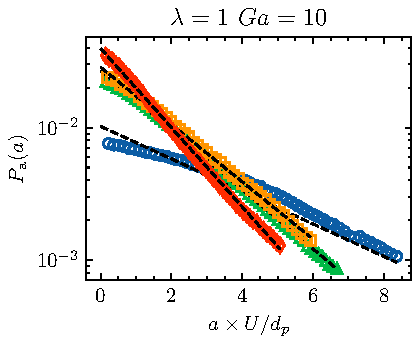
\includegraphics[height = 0.3\textwidth]{image/HOMOGENEOUS_NEW/Dist/Pa_l_1_Ga_10.pdf}
    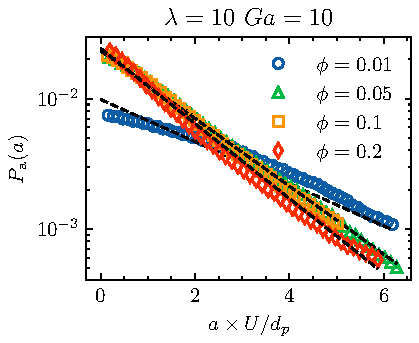
\includegraphics[height = 0.3\textwidth]{image/HOMOGENEOUS_NEW/Dist/Pa_l_10_Ga_10.pdf}
    \caption{(left) Age distribution at $\lambda = 10$ and $Ga = 10$ for : (solid line) $\phi = 0.2$; (dash dotted line) $\phi = 0.1$; (dashed line) $\phi =0.05$; (dotted line) $\phi = 0.01$. 
    (right) Mean dimensionless age in terms of the volume fraction $\phi$ for : 
    ($\bullet$) $Ga=1$; ($\blacktriangle$) $ Ga = 10$; ($\blacksquare$) $Ga = 50$ ($\blacklozenge$) $Ga =100$.
    The age and $\tau_a$ are made dimensionless with $U/d$ where $U$ is the drift-velocity between the dispersed and continuous phase.  }
    \label{fig:age_picture}
\end{figure}